\startslide
\commonframe
\mbox{}

\begin{tikzpicture}[remember picture,overlay]
  \slidetitle{Вариант на MongoDB}

  \node[anchor=north west] at ([xshift=8.40cm,yshift=-1.95cm]current page.north west) {%
    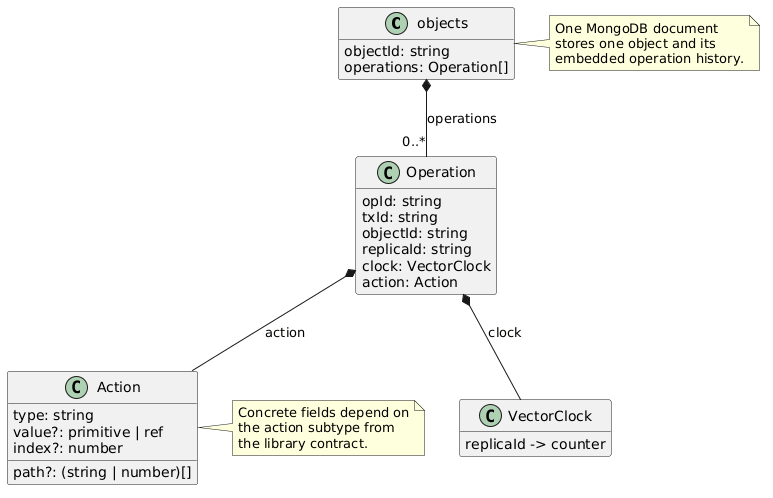
\includegraphics[width=5.70cm]{../mongodb/resources/diagram.png}%
  };

  \node[
    anchor=north west,
    fill=softrose,
    rounded corners=10pt,
    text width=6.2cm,
    inner xsep=0.35cm,
    inner ysep=0.28cm,
    align=left
  ] at ([xshift=0.95cm,yshift=-1.95cm]current page.north west) {%
    {\fontsize{9.4}{10.9}\selectfont
    \textbf{Модель хранения}\\[0.10cm]
    Одна коллекция \texttt{objects}. Каждый документ содержит
    \texttt{objectId} и массив \texttt{operations}.}%
  };

  \node[
    anchor=north west,
    fill=softgray,
    rounded corners=10pt,
    text width=6.2cm,
    inner xsep=0.30cm,
    inner ysep=0.24cm,
    align=left
  ] at ([xshift=0.95cm,yshift=-4.35cm]current page.north west) {%
    {\fontsize{9.0}{10.0}\selectfont
    \textbf{Сильные стороны}\\
    • естественное хранение \texttt{clock} и \texttt{action};\\
    • полная история объекта читается из одного документа.\\[0.16cm]
    \textbf{Ограничения}\\
    • лимит документа \texttt{16 MB};\\
    • при росте истории нужна сегментация.}%
  };

\end{tikzpicture}

\footerband{5}
